%% template.tex
%% from
%% bare_conf.tex
%% V1.4b
%% 2015/08/26
%% by Michael Shell
%% See:
%% http://www.michaelshell.org/
%% for current contact information.
%%
%% This is a skeleton file demonstrating the use of IEEEtran.cls
%% (requires IEEEtran.cls version 1.8b or later) with an IEEE
%% conference paper.
%%
%% Support sites:
%% http://www.michaelshell.org/tex/ieeetran/
%% http://www.ctan.org/pkg/ieeetran
%% and
%% http://www.ieee.org/

%%*************************************************************************
%% Legal Notice:
%% This code is offered as-is without any warranty either expressed or
%% implied; without even the implied warranty of MERCHANTABILITY or
%% FITNESS FOR A PARTICULAR PURPOSE!
%% User assumes all risk.
%% In no event shall the IEEE or any contributor to this code be liable for
%% any damages or losses, including, but not limited to, incidental,
%% consequential, or any other damages, resulting from the use or misuse
%% of any information contained here.
%%
%% All comments are the opinions of their respective authors and are not
%% necessarily endorsed by the IEEE.
%%
%% This work is distributed under the LaTeX Project Public License (LPPL)
%% ( http://www.latex-project.org/ ) version 1.3, and may be freely used,
%% distributed and modified. A copy of the LPPL, version 1.3, is included
%% in the base LaTeX documentation of all distributions of LaTeX released
%% 2003/12/01 or later.
%% Retain all contribution notices and credits.
%% ** Modified files should be clearly indicated as such, including  **
%% ** renaming them and changing author support contact information. **
%%*************************************************************************


% *** Authors should verify (and, if needed, correct) their LaTeX system  ***
% *** with the testflow diagnostic prior to trusting their LaTeX platform ***
% *** with production work. The IEEE's font choices and paper sizes can   ***
% *** trigger bugs that do not appear when using other class files.       ***                          ***
% The testflow support page is at:
% http://www.michaelshell.org/tex/testflow/

\documentclass[conference,final,]{IEEEtran}
% Some Computer Society conferences also require the compsoc mode option,
% but others use the standard conference format.
%
% If IEEEtran.cls has not been installed into the LaTeX system files,
% manually specify the path to it like:
% \documentclass[conference]{../sty/IEEEtran}





% Some very useful LaTeX packages include:
% (uncomment the ones you want to load)


% *** MISC UTILITY PACKAGES ***
%
%\usepackage{ifpdf}
% Heiko Oberdiek's ifpdf.sty is very useful if you need conditional
% compilation based on whether the output is pdf or dvi.
% usage:
% \ifpdf
%   % pdf code
% \else
%   % dvi code
% \fi
% The latest version of ifpdf.sty can be obtained from:
% http://www.ctan.org/pkg/ifpdf
% Also, note that IEEEtran.cls V1.7 and later provides a builtin
% \ifCLASSINFOpdf conditional that works the same way.
% When switching from latex to pdflatex and vice-versa, the compiler may
% have to be run twice to clear warning/error messages.






% *** CITATION PACKAGES ***
%
%\usepackage{cite}
% cite.sty was written by Donald Arseneau
% V1.6 and later of IEEEtran pre-defines the format of the cite.sty package
% \cite{} output to follow that of the IEEE. Loading the cite package will
% result in citation numbers being automatically sorted and properly
% "compressed/ranged". e.g., [1], [9], [2], [7], [5], [6] without using
% cite.sty will become [1], [2], [5]--[7], [9] using cite.sty. cite.sty's
% \cite will automatically add leading space, if needed. Use cite.sty's
% noadjust option (cite.sty V3.8 and later) if you want to turn this off
% such as if a citation ever needs to be enclosed in parenthesis.
% cite.sty is already installed on most LaTeX systems. Be sure and use
% version 5.0 (2009-03-20) and later if using hyperref.sty.
% The latest version can be obtained at:
% http://www.ctan.org/pkg/cite
% The documentation is contained in the cite.sty file itself.






% *** GRAPHICS RELATED PACKAGES ***
%
\ifCLASSINFOpdf
  % \usepackage[pdftex]{graphicx}
  % declare the path(s) where your graphic files are
  % \graphicspath{{../pdf/}{../jpeg/}}
  % and their extensions so you won't have to specify these with
  % every instance of \includegraphics
  % \DeclareGraphicsExtensions{.pdf,.jpeg,.png}
\else
  % or other class option (dvipsone, dvipdf, if not using dvips). graphicx
  % will default to the driver specified in the system graphics.cfg if no
  % driver is specified.
  % \usepackage[dvips]{graphicx}
  % declare the path(s) where your graphic files are
  % \graphicspath{{../eps/}}
  % and their extensions so you won't have to specify these with
  % every instance of \includegraphics
  % \DeclareGraphicsExtensions{.eps}
\fi
% graphicx was written by David Carlisle and Sebastian Rahtz. It is
% required if you want graphics, photos, etc. graphicx.sty is already
% installed on most LaTeX systems. The latest version and documentation
% can be obtained at:
% http://www.ctan.org/pkg/graphicx
% Another good source of documentation is "Using Imported Graphics in
% LaTeX2e" by Keith Reckdahl which can be found at:
% http://www.ctan.org/pkg/epslatex
%
% latex, and pdflatex in dvi mode, support graphics in encapsulated
% postscript (.eps) format. pdflatex in pdf mode supports graphics
% in .pdf, .jpeg, .png and .mps (metapost) formats. Users should ensure
% that all non-photo figures use a vector format (.eps, .pdf, .mps) and
% not a bitmapped formats (.jpeg, .png). The IEEE frowns on bitmapped formats
% which can result in "jaggedy"/blurry rendering of lines and letters as
% well as large increases in file sizes.
%
% You can find documentation about the pdfTeX application at:
% http://www.tug.org/applications/pdftex





% *** MATH PACKAGES ***
%
%\usepackage{amsmath}
% A popular package from the American Mathematical Society that provides
% many useful and powerful commands for dealing with mathematics.
%
% Note that the amsmath package sets \interdisplaylinepenalty to 10000
% thus preventing page breaks from occurring within multiline equations. Use:
%\interdisplaylinepenalty=2500
% after loading amsmath to restore such page breaks as IEEEtran.cls normally
% does. amsmath.sty is already installed on most LaTeX systems. The latest
% version and documentation can be obtained at:
% http://www.ctan.org/pkg/amsmath





% *** SPECIALIZED LIST PACKAGES ***
%
%\usepackage{algorithmic}
% algorithmic.sty was written by Peter Williams and Rogerio Brito.
% This package provides an algorithmic environment fo describing algorithms.
% You can use the algorithmic environment in-text or within a figure
% environment to provide for a floating algorithm. Do NOT use the algorithm
% floating environment provided by algorithm.sty (by the same authors) or
% algorithm2e.sty (by Christophe Fiorio) as the IEEE does not use dedicated
% algorithm float types and packages that provide these will not provide
% correct IEEE style captions. The latest version and documentation of
% algorithmic.sty can be obtained at:
% http://www.ctan.org/pkg/algorithms
% Also of interest may be the (relatively newer and more customizable)
% algorithmicx.sty package by Szasz Janos:
% http://www.ctan.org/pkg/algorithmicx




% *** ALIGNMENT PACKAGES ***
%
%\usepackage{array}
% Frank Mittelbach's and David Carlisle's array.sty patches and improves
% the standard LaTeX2e array and tabular environments to provide better
% appearance and additional user controls. As the default LaTeX2e table
% generation code is lacking to the point of almost being broken with
% respect to the quality of the end results, all users are strongly
% advised to use an enhanced (at the very least that provided by array.sty)
% set of table tools. array.sty is already installed on most systems. The
% latest version and documentation can be obtained at:
% http://www.ctan.org/pkg/array


% IEEEtran contains the IEEEeqnarray family of commands that can be used to
% generate multiline equations as well as matrices, tables, etc., of high
% quality.




% *** SUBFIGURE PACKAGES ***
%\ifCLASSOPTIONcompsoc
%  \usepackage[caption=false,font=normalsize,labelfont=sf,textfont=sf]{subfig}
%\else
%  \usepackage[caption=false,font=footnotesize]{subfig}
%\fi
% subfig.sty, written by Steven Douglas Cochran, is the modern replacement
% for subfigure.sty, the latter of which is no longer maintained and is
% incompatible with some LaTeX packages including fixltx2e. However,
% subfig.sty requires and automatically loads Axel Sommerfeldt's caption.sty
% which will override IEEEtran.cls' handling of captions and this will result
% in non-IEEE style figure/table captions. To prevent this problem, be sure
% and invoke subfig.sty's "caption=false" package option (available since
% subfig.sty version 1.3, 2005/06/28) as this is will preserve IEEEtran.cls
% handling of captions.
% Note that the Computer Society format requires a larger sans serif font
% than the serif footnote size font used in traditional IEEE formatting
% and thus the need to invoke different subfig.sty package options depending
% on whether compsoc mode has been enabled.
%
% The latest version and documentation of subfig.sty can be obtained at:
% http://www.ctan.org/pkg/subfig




% *** FLOAT PACKAGES ***
%

%\usepackage{fixltx2e}
% fixltx2e, the successor to the earlier fix2col.sty, was written by
% Frank Mittelbach and David Carlisle. This package corrects a few problems
% in the LaTeX2e kernel, the most notable of which is that in current
% LaTeX2e releases, the ordering of single and double column floats is not
% guaranteed to be preserved. Thus, an unpatched LaTeX2e can allow a
% single column figure to be placed prior to an earlier double column
% figure.
% Be aware that LaTeX2e kernels dated 2015 and later have fixltx2e.sty's
% corrections already built into the system in which case a warning will
% be issued if an attempt is made to load fixltx2e.sty as it is no longer
% needed.
% The latest version and documentation can be found at:
% http://www.ctan.org/pkg/fixltx2e


%\usepackage{stfloats}
% stfloats.sty was written by Sigitas Tolusis. This package gives LaTeX2e
% the ability to do double column floats at the bottom of the page as well
% as the top. (e.g., "\begin{figure*}[!b]" is not normally possible in
% LaTeX2e). It also provides a command:
%\fnbelowfloat
% to enable the placement of footnotes below bottom floats (the standard
% LaTeX2e kernel puts them above bottom floats). This is an invasive package
% which rewrites many portions of the LaTeX2e float routines. It may not work
% with other packages that modify the LaTeX2e float routines. The latest
% version and documentation can be obtained at:
% http://www.ctan.org/pkg/stfloats
% Do not use the stfloats baselinefloat ability as the IEEE does not allow
% \baselineskip to stretch. Authors submitting work to the IEEE should note
% that the IEEE rarely uses double column equations and that authors should try
% to avoid such use. Do not be tempted to use the cuted.sty or midfloat.sty
% packages (also by Sigitas Tolusis) as the IEEE does not format its papers in
% such ways.
% Do not attempt to use stfloats with fixltx2e as they are incompatible.
% Instead, use Morten Hogholm'a dblfloatfix which combines the features
% of both fixltx2e and stfloats:
%
% \usepackage{dblfloatfix}
% The latest version can be found at:
% http://www.ctan.org/pkg/dblfloatfix




% *** PDF, URL AND HYPERLINK PACKAGES ***
%
%\usepackage{url}
% url.sty was written by Donald Arseneau. It provides better support for
% handling and breaking URLs. url.sty is already installed on most LaTeX
% systems. The latest version and documentation can be obtained at:
% http://www.ctan.org/pkg/url
% Basically, \url{my_url_here}.




% *** Do not adjust lengths that control margins, column widths, etc. ***
% *** Do not use packages that alter fonts (such as pslatex).         ***
% There should be no need to do such things with IEEEtran.cls V1.6 and later.
% (Unless specifically asked to do so by the journal or conference you plan
% to submit to, of course. )



%% BEGIN MY ADDITIONS %%


\usepackage{graphicx}
% We will generate all images so they have a width \maxwidth. This means
% that they will get their normal width if they fit onto the page, but
% are scaled down if they would overflow the margins.
\makeatletter
\def\maxwidth{\ifdim\Gin@nat@width>\linewidth\linewidth
\else\Gin@nat@width\fi}
\makeatother
\let\Oldincludegraphics\includegraphics
\renewcommand{\includegraphics}[1]{\Oldincludegraphics[width=\maxwidth]{#1}}

\usepackage[unicode=true]{hyperref}

\hypersetup{
            pdftitle={The Emotional Coherence Controversy: Evidence from Human and Automatic Expression Recognition},
            pdfborder={0 0 0},
            breaklinks=true}
\urlstyle{same}  % don't use monospace font for urls

% Pandoc toggle for numbering sections (defaults to be off)
\setcounter{secnumdepth}{0}

% Pandoc syntax highlighting

% Pandoc header
\usepackage{booktabs}
\usepackage{float}
\usepackage{tabu}
\usepackage{wrapfig}
\usepackage[none]{hyphenat}
\floatplacement{figure}{H}
\usepackage{flushend}
\usepackage{biblatex}

\providecommand{\tightlist}{%
  \setlength{\itemsep}{0pt}\setlength{\parskip}{0pt}}

%% END MY ADDITIONS %%


\hyphenation{op-tical net-works semi-conduc-tor}

\begin{document}
%
% paper title
% Titles are generally capitalized except for words such as a, an, and, as,
% at, but, by, for, in, nor, of, on, or, the, to and up, which are usually
% not capitalized unless they are the first or last word of the title.
% Linebreaks \\ can be used within to get better formatting as desired.
% Do not put math or special symbols in the title.
\title{The Emotional Coherence Controversy: Evidence from Human and Automatic
Expression Recognition}

% author names and affiliations
% use a multiple column layout for up to three different
% affiliations

\author{

%% ---- classic IEEETrans wide authors' list ----------------
 % -- end affiliation.wide
%% ----------------------------------------------------------



%% ---- classic IEEETrans one column per institution --------
 %% -- beg if/affiliation.institution-columnar
\IEEEauthorblockN{
  %% -- beg for/affiliation.institution.author
Damien Dupré %% -- end for/affiliation.institution.author
}
\IEEEauthorblockA{Business School\\
Dublin City University\\
Dublin, Ireland
\\damien.dupre@dcu.ie
}
\and
\IEEEauthorblockN{
  %% -- beg for/affiliation.institution.author
Anna Tcherkassof %% -- end for/affiliation.institution.author
}
\IEEEauthorblockA{Laboratoire Inter-universitaire de Psychologie\\
Université Grenoble Alpes\\
Grenoble, France
  %% -- beg for/affiliation.institution.author
\\anna.tcherkassof@univ-grenoble-alpes.fr
 %% -- end for/affiliation.institution.author
}
 %% -- end for/affiliation.institution
 %% -- end if/affiliation.institution-columnar
%% ----------------------------------------------------------





%% ---- one column per author, classic/default IEEETrans ----
 %% -- end if/affiliation.institution-columnar
%% ----------------------------------------------------------

}

% conference papers do not typically use \thanks and this command
% is locked out in conference mode. If really needed, such as for
% the acknowledgment of grants, issue a \IEEEoverridecommandlockouts
% after \documentclass

% for over three affiliations, or if they all won't fit within the width
% of the page, use this alternative format:
%
%\author{\IEEEauthorblockN{Michael Shell\IEEEauthorrefmark{1},
%Homer Simpson\IEEEauthorrefmark{2},
%James Kirk\IEEEauthorrefmark{3},
%Montgomery Scott\IEEEauthorrefmark{3} and
%Eldon Tyrell\IEEEauthorrefmark{4}}
%\IEEEauthorblockA{\IEEEauthorrefmark{1}School of Electrical and Computer Engineering\\
%Georgia Institute of Technology,
%Atlanta, Georgia 30332--0250\\ Email: see http://www.michaelshell.org/contact.html}
%\IEEEauthorblockA{\IEEEauthorrefmark{2}Twentieth Century Fox, Springfield, USA\\
%Email: homer@thesimpsons.com}
%\IEEEauthorblockA{\IEEEauthorrefmark{3}Starfleet Academy, San Francisco, California 96678-2391\\
%Telephone: (800) 555--1212, Fax: (888) 555--1212}
%\IEEEauthorblockA{\IEEEauthorrefmark{4}Tyrell Inc., 123 Replicant Street, Los Angeles, California 90210--4321}}




% use for special paper notices
%\IEEEspecialpapernotice{(Invited Paper)}




% make the title area
\maketitle

% As a general rule, do not put math, special symbols or citations
% in the abstract
\begin{abstract}
While it has been taken for granted in the development of several
automatic facial expression recognition tools, the question of the
coherence between subjective feelings and facial expressions is still a
subject of debate. On one hand, the behaviorist approach conceives
emotions as genetically hardwired and therefore being genuinely
displayed through facial expressions. On the other hand, the
constructivist approach conceives emotions as socially constructed; the
emotional meaning of a facial expression being inferred by the observer.
In order to evaluate the coherence between the subjective feeling of
emotions and their recognition based on facial expression, 232 videos of
encoders recruited to carry out an emotion elicitation task were
annotated by 1383 human observers as well as by an automatic facial
expression classifier. Results show low accuracy of human observers and
of the automatic classifier to infer the subjective feeling from the
facial expressions displayed by encoders. They also show a weak
coherence between self-reported emotional states and facial emotional
displays. Based on these results, the hypothesis of genetically
hardwired emotion genuinely displayed is difficult to support, whereas
the idea of emotion and facial expression socially constructed appears
to be more likely. Accordingly, automatic emotion recognition tools
based on facial expressions should be questioned.
\end{abstract}

% no keywords

% use for special paper notices



% make the title area
\maketitle

% no keywords

% For peer review papers, you can put extra information on the cover
% page as needed:
% \ifCLASSOPTIONpeerreview
% \begin{center} \bfseries EDICS Category: 3-BBND \end{center}
% \fi
%
% For peerreview papers, this IEEEtran command inserts a page break and
% creates the second title. It will be ignored for other modes.
\IEEEpeerreviewmaketitle


\begin{IEEEkeywords}
Facial expression, self-report, human observer, automatic recognition.
\end{IEEEkeywords}

\hypertarget{i.-introduction}{%
\section{I. Introduction}\label{i.-introduction}}

With the development of commercial automatic facial expression
recognition tools {[}1{]}, industries and governments are gradually
implementing this technology in order to track humans' emotions in
various scenarios (\emph{e.g.}, in marketing, healthcare, and the
automotive industry to name a few). This technology rests on the premise
that facial expressions provide a direct access to individuals'
subjective feelings also called ``emotional coherence''. Even if this
premise is central to the modern mainstream approach of human emotion,
recent research in affective science is challenging it. Once the two
competing approaches are briefly described along with the predictions
they respectively entail, an experiment testing these hypotheses will be
presented and its results analyzed in order to provide empirical
evidence to contribute to answer the question.

\hypertarget{a.-the-behaviorist-approach}{%
\subsection{A. The Behaviorist
Approach}\label{a.-the-behaviorist-approach}}

Based on the behaviorist approach initiated by Darwin in \emph{The
Expression of the Emotions in Man and Animals} {[}2{]}, facial
expressions are conceived as a genuine displays of an individual's inner
emotional state. This hypothesis is used as a basis for the Basic
Emotion Theory (BET) which states that a set of six emotions are
universally displayed and are genetically hardwired not only in humans
{[}3{]} but also in different animal species {[}4{]}. According to this
view, \emph{``when emotions are aroused by perception of a social event,
a set of central commands produce patterned emotion-specific changes in
multiple systems, including {[}\ldots{}{]} facial expressions.''} {[}5,
p. 49{]}. To respond to criticisms, several amendments have been made to
the BET, increasing the number of basic emotions from six to seven
{[}6{]} as well as adding the concept of ``display rules'' to explain
cultural differences in the management of facial expressions {[}7{]}.

Even if this theory obtained popular support, it fails to explain how
individuals can feel emotions without expressing them, and how
individuals can express emotions without feeling them, in instances in
which display rules cannot be called upon {[}8{]}, {[}9{]}. These
evidences have led to an alternative conception, notably the social
constructivist approach.

\hypertarget{b.-the-social-constructivist-approach}{%
\subsection{B. The Social Constructivist
Approach}\label{b.-the-social-constructivist-approach}}

Detractors of the Basic Emotion Theory consider emotion not as
genetically hardwired but as a learnt association between a given
situation and an appropriate response {[}10{]}, {[}11{]}. For the
proponents of the constructivist approach, emotions are ``concepts''
based on past experiences and which are \emph{``a collection of
embodied, whole brain representations that predict what is about to
happen in the sensory environment, what the best action is to deal with
impending events, and their consequences for allostasis''} {[}12, p.
12{]}. Following this assumption, faces are best conceived as tools
displaying signals in social interactions {[}13{]}. These signals can
convey individuals' motivations and readiness {[}14{]} or social
messages {[}15{]}. Therefore, facial expressions are thought as
behaviors which meaning is inferred by the observer. Findings support
this observer dependence {[}16{]}, {[}17{]}. They show that to make
meaning of another person's facial behavior, the perceiver relies in
particular on her/his knowledge about emotion categories.

\hypertarget{c.-emotional-facial-expression-recognition}{%
\subsection{C. Emotional Facial Expression
Recognition}\label{c.-emotional-facial-expression-recognition}}

Regarding emotional facial expression (EFE) recognition, behaviorist and
constructivist approaches lead to two divergent predictions. The former
postulates that, when triggered, each basic emotion is expressed by a
prototypical face (non basic emotions being blends of the basic ones).
Basic emotions are easily recognized by all human observers and
emotional states are accessible by facial measurement. As the
recognition of facial expressions is based on the identification of
specific patterns of facial movements, it implies that EFE recognition
of both human observers and automatic classifiers should be as accurate.
The constructivist approach, in contrast, affirms that facial
expressions do not provide a direct access to individuals' subjective
feelings. Even if the face possibly moves during an emotional episode,
facial muscle movements are not linked in a one-to-one manner to a
specific discrete emotional experience {[}18, p. p418{]}. Instead,
emotions are mentally constructed by the perceiver and mental categories
of emotions are needed to accurately categorize facial movements.
Therefore, since there is no emotional prototypical face, one should
expect human observers' superior ability to accurately recognize EFE as
compared to automatic EFE recognition tools (Figure
\ref{fig:models_img}).

\begin{figure}
\centering
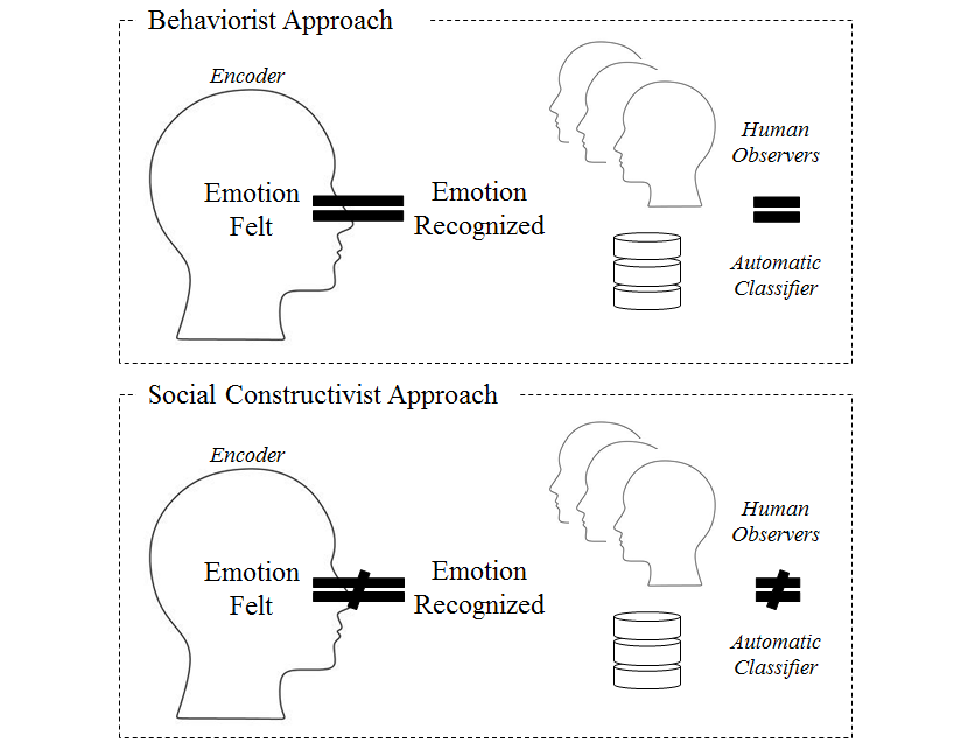
\includegraphics{ACII_2019_paper_files/figure-latex/models_img-1.pdf}
\caption{\label{fig:models_img}Comparison of behaviorist and social
constructivist approaches according to the expected differences in
emotion recognition.}
\end{figure}

The aim of the current paper is to investigate the coherence between the
subjective feeling of emotions and its recognition from facial
expressions in order to give credit either to the behaviorist plea or to
the constructivist's one. Contrary to most studies using posed and
static EFE, the present study focuses on natural EFE. Spontaneous and
dynamic facial reactions to emotional elicitations are under
consideration to ensure the generalizability of the results to emotional
behaviors in ordinary life.

\hypertarget{ii.-method}{%
\section{II. Method}\label{ii.-method}}

To evaluate the coherence between subjective feeling of emotions and
their recognition from facial expressions, encoders were first recruited
to perform an emotion elicitation task while their facial expression was
video recorded. Then, the videos of the encoders' faces were shown to
human observers and were also analysed by an automatic classifier in
order to identify which emotion was displayed.

\hypertarget{a.-emotion-elicitation}{%
\subsection{A. Emotion Elicitation}\label{a.-emotion-elicitation}}

For the emotion elicitation experiment, 358 French participants (182
females, 176 males, \emph{M}\textsubscript{age} = 47.9,
\emph{SD}\textsubscript{age} = 9.2) were recruited to perform one out of
11 emotion elicitation tasks designed to trigger a positive, a specific
negative or a neutral emotional state. Encoders' face were recorded
using an hidden camera resulting 358 front facing 768x576 videos varying
from 1s to 1479s (Figure \ref{fig:dynemo_img}). These recordings form
the DynEmo database {[}19{]}.

\begin{figure}
\centering
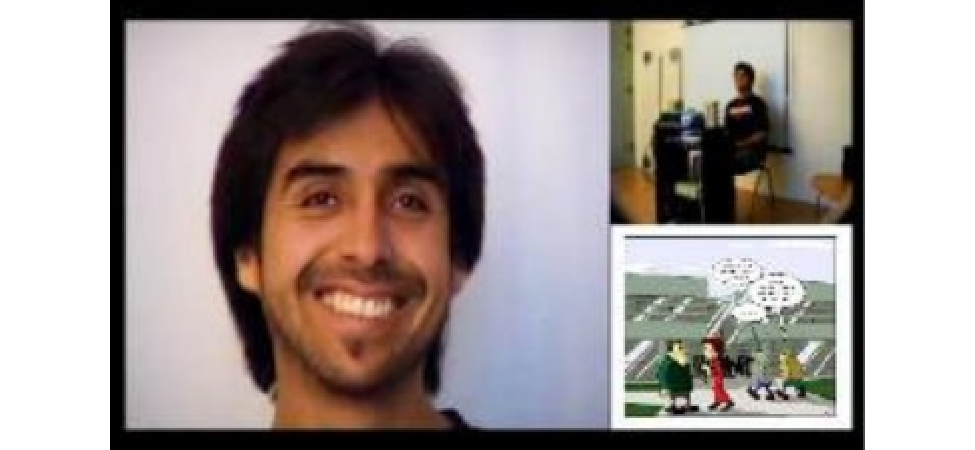
\includegraphics{ACII_2019_paper_files/figure-latex/dynemo_img-1.pdf}
\caption{\label{fig:dynemo_img}Example of a front facing recording
synced with the full view of the participant and the elicitation task.
This picture is taken from a pilot with projects collaborators and all
gave consent for the publication of their photos and videos.}
\end{figure}

After the emotion elicitation task the encoders rated their subjective
feeling on Likert scales from 0 (``not at all'') to \nolinebreak 5
\nolinebreak (``strongly'') related to six ``basic'' emotion labels
(\emph{i.e.}, \emph{anger}, \emph{disgust}, \emph{fear},
\emph{happiness}, \emph{surprise} and \emph{sadness}) as well as six
``non-basic'' emotion labels (\emph{i.e.}, \emph{pride},
\emph{curiosity}, \emph{boredom}, \emph{shame}, \emph{humiliation}, and
\emph{disappointment}).

Finally, a debriefing session was performed to ensure that encoders were
not durably affected by the emotion elicitation task. The debriefing was
also used to check that encoders did not guess the real purpose of the
experiment (\emph{e.g.}, being filmed while they were performing an
emotional elicitation task) to guarantee facial expressions'
genuineness. All encoders gave their agreement on their data and video
to be processed for research purposes only.

\hypertarget{b.-human-facial-expression-recognition}{%
\subsection{B. Human Facial Expression
Recognition}\label{b.-human-facial-expression-recognition}}

For the human facial expression recognition method, 1383
\nolinebreak student participants were recruited to annotate 232 out of
the 358 videos, therefore only the 232 annotated videos will be analysed
in this paper. Because videos have different durations, participants had
to annotate a series of video corresponding to 30min long in total. Each
video was annotated 29 times on average (\emph{SD} = 12).

The annotation of facial expressions was performed on-site using
\emph{Oudjat}, a software for designing video annotation experiments
{[}20{]}. For each video, the annotation procedure followed two steps.
First, the participants had to identify the emotional sequences by
pressing the space bar of their keyboard to indicate the beginning and
the end of the emotional sequences while watching the video. Second, the
participants watched each emotional sequence previously identified and
labeled the sequence using one of the 12 \nolinebreak emotions proposed
including six ``basic'' emotion labels (\emph{i.e.}, \emph{anger},
\emph{disgust}, \emph{fear}, \emph{happiness}, \emph{surprise} and
\emph{sadness}) and six ``non-basic'' emotion labels (\emph{i.e.},
\emph{pride}, \emph{curiosity}, \emph{boredom}, \emph{shame},
\emph{humiliation}, and \emph{disappointment}). They also had the
possibility to indicate that the sequence was expressing none of the
proposed emotion labels.

This annotation procedure results in a uni-dimensional time-series for
each video per human observer identifying for each second of the video
which emotion was recognized. Then, time-series corresponding to the
same video were aggregated to calculate the proportion of human
observers \(x_{video_{i}.label_{j}.t_{k}}\) for each second of the video
per emotional label (EQ\ref{eq:1}).

\begin{equation}
\label{eq:1}
x_{video_{i}.label_{j}.t_{k}} = \frac{n_{video_{i}.label_{j}.t_{k}}}{n_{video_{k}}}
\end{equation}

where \emph{i} is one of the 232 videos, \emph{j} is one of the six
``basic'' emotion labels, \emph{k} for each second of the video.

\hypertarget{c.-automatic-facial-expression-recognition}{%
\subsection{C. Automatic Facial Expression
Recognition}\label{c.-automatic-facial-expression-recognition}}

The 232 annotated video were processed with Affdex (SDK v3.4.1). Affdex
is an automatic facial expression recognition classifier developed and
distributed by Affectiva is a spin-off company resulting from the
research activities of MIT media lab created in 2009 {[}21{]}. Affdex's
algorithm uses Histogram of Oriented Gradient (HOG) features and Support
Vector Machine (SVM) classifiers in order to recognize facial
expressions. For each video frame, Affdex identifies the probability
\(p_{video_{i}.label_{j}.t_{k}}\) from 0 to 100 (rescaled to 0 to 1 for
the analysis) of the face as expressing one of the six ``basic'' emotion
labels (\emph{i.e.}, \emph{anger}, \emph{disgust}, \emph{fear},
\emph{happiness}, \emph{surprise} and \emph{sadness}) as well as
additional psychological states such as \emph{valence},
\emph{engagement} or \emph{contempt}, and facial features such as
\emph{cheek raise}, \emph{eye widen} or \emph{jaw drop}.

For both human and automatic recognition, to determine which of the six
``basic'' emotions can be used to identify each video, the recognition
probability for each label by frame was converted into odd ratio by
label {[}22{]}. The highest sum of each odd ratio time-series defines
the label recognized by the automatic classifier (EQ\ref{eq:2} for human
recognition and EQ\ref{eq:3} for automatic recognition).
\begin{equation}
\label{eq:2}
video_{i}.label = \max\left(\frac{\sum_{k=1}^{n}x_{video_{i}.label_{j}.t_{k}}}{\sum_{k=1}^{n}x_{video_{i}.t_{k}}}\right)
\end{equation}

\begin{equation}
\label{eq:3}
video_{i}.label = \max\left(\frac{\sum_{k=1}^{f}p_{video_{i}.label_{j}.t_{k}}}{\sum_{k=1}^{f}p_{video_{i}.t_{k}}}\right)
\end{equation}

where \emph{i} is one of the 232 videos, \emph{j} is one of the six
``basic'' emotion labels, \emph{k} for each second of the \emph{n}
second video or for each frame of the \emph{f} frame video.

\hypertarget{iii.-results}{%
\section{III. Results}\label{iii.-results}}

Since encoders' self-reports, human annotations and the automatic
recognition include data on ``non-basic'' emotion labels and features,
the analysis is performed using only the six ``basic'' emotion labels in
order to compare them. The maximum score for self-reports, human
annotations and automatic recognition is used to label the video. In
case of more than one label obtaining the maximum value, the video is
labeled as undetermined.

\hypertarget{a.-human-observers-accuracy}{%
\subsection{A. Human Observers'
Accuracy}\label{a.-human-observers-accuracy}}

The overall correlation of recognition and non-recognition between
self-reported emotions and human observers recognition is significant
but low (\(r = .24\), 95\% CI \([.19\), \(.29]\), \(t(1384) = 9.21\),
\(p < .001\)). In order to identify differences according to the
emotional labels, encoders' subjective feelings are compared with human
observers' recognition in a confusion matrix (Figure
\ref{fig:confusionMatrix_sr_hr}).

\begin{figure}
\centering
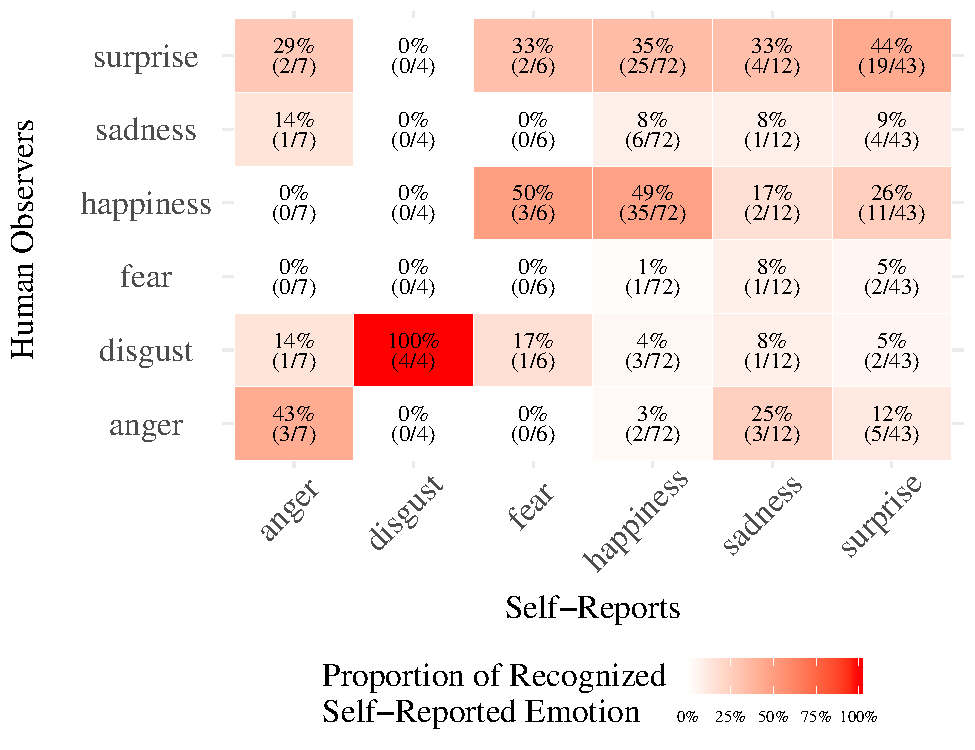
\includegraphics{ACII_2019_paper_files/figure-latex/confusionMatrix_sr_hr-1.pdf}
\caption{\label{fig:confusionMatrix_sr_hr}Confusion matrix between the
emotion self-reported as being characteristic of the elicitation with
the emotion recognized by the human observers.}
\end{figure}

Each emotion label used to describe encoders' self-reported subjective
feeling (\emph{i.e.}, the label rated with the highest value) is
compared with the emotion labels which were rated with the highest score
by human observers. Results of the confusion matrix show a moderate
agreement between the emotion felt by the encoder during the elicitation
and the emotion recognized by the human observers (Accuracy
\nolinebreak = \nolinebreak 0.43, 95\% CI {[}0.35,0.52{]}; Kappa = 0.19)
except for \emph{disgust} (100\% of the videos self-reported). These
results are far from those classically obtained in the literature for
emotional facial expression recognition which ranges between 60\% and
80\% accuracy. However these results are mostly obtained with static
(\emph{i.e.,} pictures) and posed (\emph{i.e.,} displayed by actors)
facial expressions using only 6 emotional labels in a forced-choice
paradigm.

Interestingly human observers seem to recognize \emph{surprise}
expressed in videos where \emph{anger}, \emph{fear} \emph{happiness} and
\emph{sadness} was the highest self-reported emotion (respectively
28.6\%, 33.3\%, 34.7\% and 33.3\% of the videos self-reported), and in a
lower instance \emph{happiness} was recognized in videos where
\emph{fear} and \emph{surprise} was the highest self-reported emotion
(respectively 50.0\% and 25.6\% of the videos self-reported).

Sensitivity, specificity, precision and F1 scores for each emotion
reveals that \emph{happiness} has the highest coherence ratio whereas
\emph{sadness} has the lowest coherence ratio between true positives and
false positives (Table \ref{table:confusionTable_sr_hr}).

\begin{table}[H]

\caption{\label{tab:confusionTable_sr_hr}\label{table:confusionTable_sr_hr}Human recognition accuracy metrics for each emotion.}
\centering
\fontsize{8}{10}\selectfont
\begin{tabu} to \linewidth {>{\raggedright}X>{\centering}X>{\centering}X>{\centering}X>{\centering}X}
\toprule
Emotion & Sensitivity & Specificity & Precision & F1\\
\midrule
anger & 0.43 & 0.93 & 0.23 & 0.3\\
disgust & 1.00 & 0.94 & 0.33 & 0.5\\
fear & 0.00 & 0.97 & 0.00 & \textit{na.}\\
happiness & 0.49 & 0.78 & 0.69 & 0.57\\
sadness & 0.08 & 0.92 & 0.08 & 0.08\\
surprise & 0.44 & 0.67 & 0.37 & 0.4\\
\bottomrule
\multicolumn{5}{l}{\textsuperscript{} Note. \textit{na.} values are produced when not enough}\\
\multicolumn{5}{l}{data are available to compute accuracy indicators.}\\
\end{tabu}
\end{table}

Accuracy metrics by emotional labels indicate a discrepancy in the ratio
of true/false positives. Whereas \emph{happiness} and \emph{disgust}
obtain the highest scores, \emph{anger}, \emph{surprise} and
\emph{sadness} have the lowest recognition ratio. The underlying effect
of expression intensity may explain why \emph{happiness} and
\emph{disgust} are easily recognized. \emph{Anger} and \emph{sadness} as
non-socially desirable emotions may be have been felt but not expressed.

However, self-reports show a significant proportion of undetermined
emotional states (35.2\% of the 358 videos) which reveals the potential
limit of using 6-points likert scales to measure emotional self-reports.
Indeed, encoders can easily score to the maximum for more than one
emotion.

\hypertarget{b.-automatic-classifiers-accuracy}{%
\subsection{B. Automatic Classifier's
Accuracy}\label{b.-automatic-classifiers-accuracy}}

Similarly to the previous analysis, the overall correlation of
recognition and non-recognition revealed a significant but very low
coherence between self-reported emotions and automatic
\nolinebreak classifier's recognition (\(r = .12\), 95\% CI \([.07\),
\(.17]\), \(t(1384) = 4.50\), \(p < .001\)). A confusion matrix was used
to compare encoders' subjective feeling with the emotion label
recognized by the automatic classifier (Figure
\ref{fig:confusionMatrix_sr_ar}).

\begin{figure}
\centering
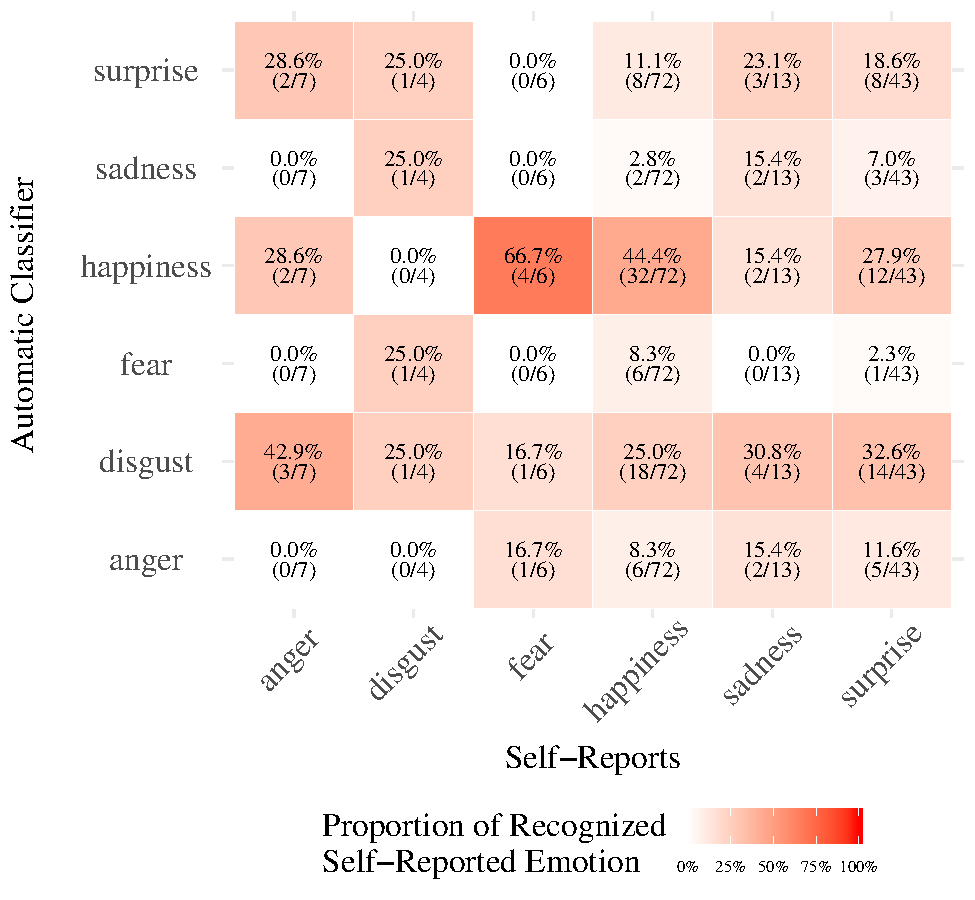
\includegraphics{ACII_2019_paper_files/figure-latex/confusionMatrix_sr_ar-1.pdf}
\caption{\label{fig:confusionMatrix_sr_ar}Confusion matrix of between
the emotion self-reported as being characteristic of the elicitation
with the emotion recognized by the automatic classifier.}
\end{figure}

Results obtained for the comparison between emotions self-reported and
recognized by the automatic classifier are somewhat similar to the ones
with human observers (Table
\nolinebreak \ref{table:confusionTable_sr_ar}). Overall, a low agreement
between emotion self-reported and emotion recognized by the automatic
classifier (Accuracy \nolinebreak = \nolinebreak 0.3, 95\% CI
{[}0.22,0.38{]}; Kappa \nolinebreak = \nolinebreak 0.07) except for
\emph{happiness} (44.4\% of the video self-reported) is evident.

Surprisingly the automatic classifier incorrectly recognized as
\emph{disgust} an significant proportion of videos in which
\emph{anger}, \emph{happiness} and \emph{surprise} was the highest
self-reported emotion (respectively 42.9\%, 25.0\% and 32.6\% of the
videos self-reported). In parallel, the automatic classifier recognized
as \emph{happiness} videos in which \emph{fear} and \emph{surprise} was
the highest self-reported emotion (respectively 66.7\% and 32.6\% of the
videos self-reported).

\begin{table}[H]

\caption{\label{tab:confusionTable_sr_ar}\label{table:confusionTable_sr_ar}Autonatic recognition accuracy metrics for each emotion.}
\centering
\fontsize{8}{10}\selectfont
\begin{tabu} to \linewidth {>{\raggedright}X>{\centering}X>{\centering}X>{\centering}X>{\centering}X}
\toprule
Emotion & Sensitivity & Specificity & Precision & F1\\
\midrule
anger & 0.00 & 0.90 & 0.00 & \textit{na.}\\
disgust & 0.25 & 0.72 & 0.02 & 0.04\\
fear & 0.00 & 0.94 & 0.00 & \textit{na.}\\
happiness & 0.44 & 0.73 & 0.62 & 0.52\\
sadness & 0.15 & 0.95 & 0.25 & 0.19\\
surprise & 0.19 & 0.86 & 0.36 & 0.25\\
\bottomrule
\multicolumn{5}{l}{\textsuperscript{} Note. \textit{na.} values are produced when not enough}\\
\multicolumn{5}{l}{data are available to compute accuracy indicators.}\\
\end{tabu}
\end{table}

A comparable explanation involving the amount of undetermined video
based on self-reports can be provided, as the level of undetermined
emotions are very high for the self reports.

\hypertarget{c.-comparison-between-human-and-automatic-recognition}{%
\subsection{C. Comparison Between Human and Automatic
Recognition}\label{c.-comparison-between-human-and-automatic-recognition}}

As previously mentioned, human observers appear to be more accurate than
the automatic classifier to recognize an individual's subjective feeling
(human observers Accuracy \nolinebreak = \nolinebreak0.43; automatic
classifier Accuracy = 0.3; \(r = .22\), 95\% CI \([.17\), \(.27]\),
\(t(1384) = 8.31\), \(p < .001\)). However, both make mistakes.

A third confusion matrix is used to compare similarities (diagonal) and
differences between human observers and automatic classifier in
classifing the six emotion labels (Figure
\nolinebreak \ref{fig:confusionMatrix_hr_ar}).

\begin{figure}
\centering
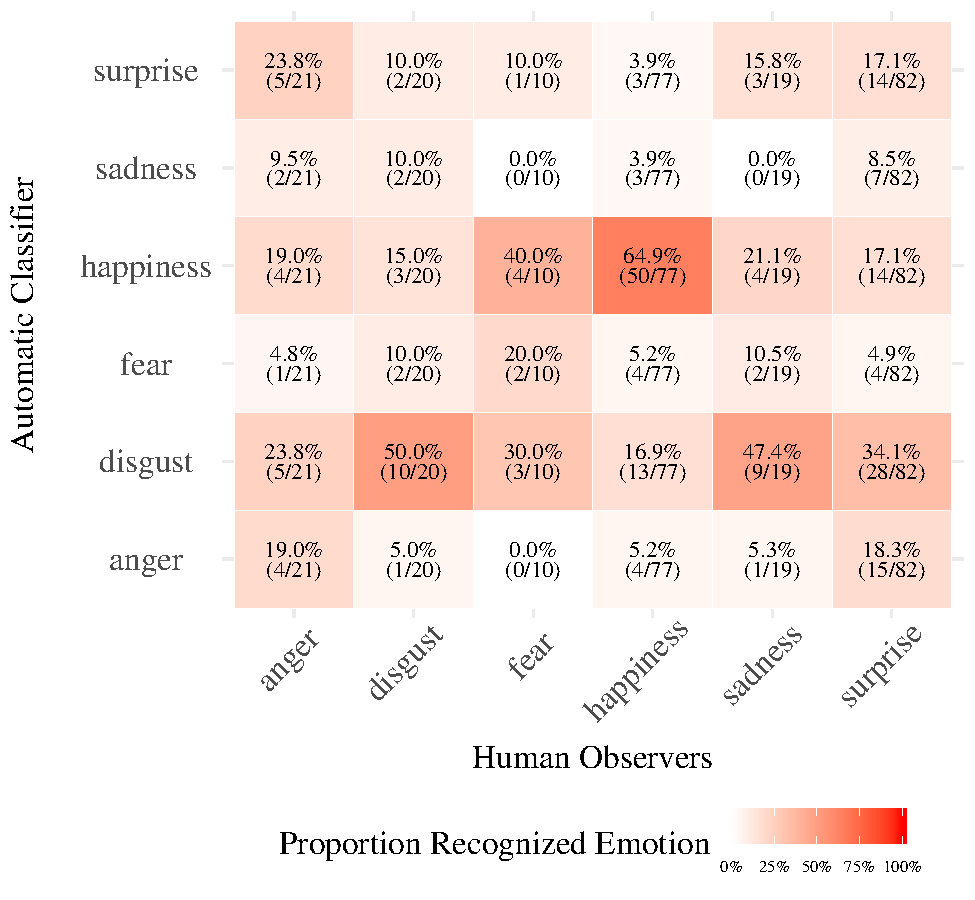
\includegraphics{ACII_2019_paper_files/figure-latex/confusionMatrix_hr_ar-1.pdf}
\caption{\label{fig:confusionMatrix_hr_ar}Proportion of emotion labels
classified by human observers which are recognized by the automatif
classifier.}
\end{figure}

The overall agreement between human observers and the automatic
classifier is in fact very low (Kappa = 0.18). Except for
\emph{happiness} and \emph{disgust} (respectively 64.9\% and 50.0\% of
common labelling), there is no clear common pattern. Moreover, the
automatic classifier has a tendency to label as \emph{disgust} videos
labeled as \emph{sadness} by human observers, and as \emph{happiness}
videos labeled as \emph{fear} by human observers.

\hypertarget{iv.-discussion-and-conclusion}{%
\section{IV. Discussion and
Conclusion}\label{iv.-discussion-and-conclusion}}

Despite being one of the most investigated questions in affective
science, the coherence between emotion felt and facially displayed on
the one hand, and facial expression recognized on the other is a hot
topic. To date no clear evidence has been found to definitively solve
the questions raised. Yet, with the growing interest of industries and
government in monitoring individual's psychological states, this issue
is under intense scrutiny. The present research aims to provide some
empirical data to answer some of the questions posed. The faces encoders
displayed when confronted with an emotional eliciting task were
submitted both to human and to automatic recognition. The criterion for
recognition accuracy was the subjective feeling self-reported by the
encoder once the elicitation task was carried out. Results first reveal
a low coherence between emotion felt and facial expression displayed.
Secondly, results show low accuracy rates for both humans and the
automatic classifier in identifying the inner emotional states of these
encoders based on their facial expressions. Thirdly, human observers
prove to be better at recognizing the emotion facially expressed than
the automatic recognition tool is.

Such results support the hypothesis advanced by some authors of a low
emotion--expression coherence {[}23{]}. In many instances, facial
displays are not associated with a concordant emotional state, even any
emotional state at all {[}24{]}, {[}25{]}. More and more evidence is
showing that facial expressions are in reality not expressing emotions
{[}26{]}. As well as other nonverbal behaviors, facial movements are not
only assumed to be determined by emotion but also by various other
causes, such as psychological states (\emph{e.g.},
\nolinebreak motivations or pain), to say nothing of social context and
sociocultural norms {[}7{]}. This multiple determination excludes any
possibility of drawing an inference from facial activity on the
underlying psychological state (emotional or other).

Beyond the present observations showing a weak coherence between
subjective feelings and spontaneous facial expressions, this study sheds
some light on the controversy between the behaviorist and the
constructivist approaches. The first of those two lines of thinking
{[}3{]} assumes that expressions of emotion are brief and coherent
patterns of facial muscle movements that co-vary with discrete
subjective experiences. Emotions and their related prototypical facial
behavior are universal because they are considered as innate mechanisms
allowing individuals to respond adaptively to evolutionary significant
events (threats, opportunities\ldots{}) encountered in the environment.
Instead of viewing emotions as natural kinds {[}12{]}, the
constructivist approach supposes that emotions are social constructions.
The specific emotion categories identified on the face of another person
are the result of categorization. In other words, the emotions that are
recognized by the observer are constructed in her/his mind, primarily
based on her/his conceptual knowledge of emotion. Therefore, facial
movements do not express specific emotions. It is the observer that
infers the emotional meaning of the facial expression. As a consequence,
one can predict from the first line of thinking that individuals'
emotional subjective feeling should be correlated to the recognition of
facial expressions from both human observers and automatic classifiers
whereas if emotions are social constructs, as stated by the second line
of thinking, human observer's should be better at perceiving emotions
expressed on the face than automatic classifiers.

Present results plead in favor of the latter stance. They show that
human observers are more accurate than the automatic recognition tool to
identify an individual's subjective feeling on the basis of their face.
Moreover, mistakes made by human observers look less arbitrary to the
ones made by the classifier. For instance, even if a mix-up between
disgust and anger is sometimes reported in recognition studies,
confusions such as the ones produced by the classifier have never been
noted for human observers. A possible explanation is that human
observers are assessing dynamic expressive sequences. They have access
to the full video which provides a kinetic context whereas the automatic
classifier only assesses the videos frame by frame. Further research is
needed to shed light on this issue.

Some limitations should be stated, notably regarding the use of
self-reports to evaluate encoders' subjective feelings. Accessing the
inner subjective feeling can be biased if not impossible. Moreover the
procedure used for human observation can also be open to dispute.
Instead of asking the human annotators to provide a unique label, a more
subtle approach was chosen to mimic results provided by the automatic
classifier. Whereas this paradigm is longer and more complicated, it can
lead to more robust results in reducing the forced-choice bias {[}27{]}.
However this procedure can also reduce the human observers' accuracy. In
this regard, the results of the human observation could have been more
ambiguous because it is not the natural way that people are inferring
meaning from facial expressions. An alternative explanation relies in
reducing the recognition bias involved in the classic recognition
paradigm. Classic forced-choice paradigms obtain artificially high
results, thus by using a more evolved approach observers' accuracy may
have been lowered.

Considering the above, the results provide additional evidence that an
individual's subjective feeling can not be inferred from facial
expressions and in our case invalidate the hypothesis of hardwired
emotions unambiguously displayed on the face. Even if emotions were
hardwired, in everyday life one does not observe prototypical facial
expressions and therefore research should be focused on analysing
non-prototypical facial expressions. Advancements in identifying
``non-basic'' emotion labels {[}28{]} as well as non-prototypical facial
expression have been made in the development of automatic facial
expression recognition tools. However, these results suggest that
automatic facial expression recognition tools should merely evaluate
facial morphology features such as action units (already evaluated in
OpenFace {[}29{]}, Affectiva's Affdex {[}21{]} or Vicar Vision's
FaceReader {[}30{]} to name a few) rather than inferring supposedly
emotional or affective states.

\hypertarget{acknowledgment}{%
\section{V. Acknowledgment}\label{acknowledgment}}

The authors would like to thank Brigitte Meillon and Jean Michel Adam
who developed the software used to collect and preprocess human observer
results.

\hypertarget{references}{%
\section{VI. References}\label{references}}

\footnotesize

\hypertarget{refs}{}
\leavevmode\hypertarget{ref-dupre2018accuracy}{}%
{[}1{]} D. Dupré, N. Andelic, G. Morrison, and G. McKeown, ``Accuracy of
three commercial automatic emotion recognition systems across different
individuals and their facial expressions,'' in \emph{Proceedings of the
international conference on pervasive computing and communications},
2018, pp. 627--632.

\leavevmode\hypertarget{ref-darwin1872expression}{}%
{[}2{]} C. Darwin, \emph{The expression of the emotions in man and
animals}. London, UK: John Murray, 1872.

\leavevmode\hypertarget{ref-ekman1992argument}{}%
{[}3{]} P. Ekman, ``An argument for basic emotions,'' \emph{Cognition \&
emotion}, vol. 6, nos. 3-4, pp. 169--200, 1992.

\leavevmode\hypertarget{ref-de2019mama}{}%
{[}4{]} F. de Waal, \emph{Mama's last hug: Animal emotions and what they
teach us about ourselves}. London, UK: Granta Books, 2019.

\leavevmode\hypertarget{ref-ekman2007directed}{}%
{[}5{]} P. Ekman, ``The directed facial action task,'' in \emph{Handbook
of emotion elicitation and assessment}, J. A. Coan and J. J. B. Allen,
Eds. New York, NY: Oxford University Press, 2007, pp. 47--53.

\leavevmode\hypertarget{ref-ekman1988universality}{}%
{[}6{]} P. Ekman and K. G. Heider, ``The universality of a contempt
expression: A replication,'' \emph{Motivation and Emotion}, vol. 12, no.
3, pp. 303--308, 1988.

\leavevmode\hypertarget{ref-ekman1987universals}{}%
{[}7{]} P. Ekman \emph{et al.}, ``Universals and cultural differences in
the judgments of facial expressions of emotion,'' \emph{Journal of
Personality and Social Psychology}, vol. 53, no. 4, pp. 712--717, 1987.

\leavevmode\hypertarget{ref-kraut1979social}{}%
{[}8{]} R. E. Kraut and R. E. Johnston, ``Social and emotional messages
of smiling: An ethological approach,'' \emph{Journal of Personality and
Social Psychology}, vol. 37, no. 9, pp. 1539--1553, 1979.

\leavevmode\hypertarget{ref-duran2017coherence}{}%
{[}9{]} J. I. Durán, R. Reisenzein, and J.-M. Fernández-Dols,
``Coherence between emotions and facial expressions,'' pp. 107--129,
2017.

\leavevmode\hypertarget{ref-averill1980constructivist}{}%
{[}10{]} J. R. Averill, ``A constructivist view of emotion,'' in
\emph{Theories of emotion}, R. Plutchik and H. Kellerman, Eds. New York,
NY: Academic Press, 1980, pp. 305--339.

\leavevmode\hypertarget{ref-barrett2017emotions}{}%
{[}11{]} L. F. Barrett, \emph{How emotions are made: The secret life of
the brain}. Boston, MA: Houghton Mifflin Harcourt, 2017.

\leavevmode\hypertarget{ref-barrett2017theory}{}%
{[}12{]} L. F. Barrett, ``The theory of constructed emotion: An active
inference account of interoception and categorization,'' \emph{Social
Cognitive and Affective Neuroscience}, vol. 12, no. 1, pp. 1--23, 2017.

\leavevmode\hypertarget{ref-crivelli2018facial}{}%
{[}13{]} C. Crivelli and A. J. Fridlund, ``Facial displays are tools for
social influence,'' \emph{Trends in Cognitive Sciences}, vol. 22, no. 5,
pp. 388--399, 2018.

\leavevmode\hypertarget{ref-frijda1997facial}{}%
{[}14{]} N. H. Frijda and A. Tcherkassof, ``Facial expressions as modes
of action readiness,'' in \emph{The psychology of facial expression}, J.
A. Russell and J.-M. Fernández-Dols, Eds. Cambridge, UK: Cambridge
University Press, 1997, pp. 78--102.

\leavevmode\hypertarget{ref-fridlund1994human}{}%
{[}15{]} A. J. Fridlund, \emph{Human facial expression: An evolutionary
view}. San Diego, CA: Academic Press, 1994.

\leavevmode\hypertarget{ref-lindquist2013s}{}%
{[}16{]} K. A. Lindquist and M. Gendron, ``What's in a word? Language
constructs emotion perception,'' \emph{Emotion Review}, vol. 5, no. 1,
pp. 66--71, 2013.

\leavevmode\hypertarget{ref-niedenthal2017embodied}{}%
{[}17{]} P. M. Niedenthal, A. Wood, M. Rychlowska, and S. Korb,
``Embodied simulation in decoding facial expression,'' in \emph{The
science of facial expression}, J.-M. Fernández-Dols and J. A. Russell,
Eds. New York, NY: Oxford University Press, 2017, pp. 397--414.

\leavevmode\hypertarget{ref-doyle2017language}{}%
{[}18{]} C. M. Doyle and K. A. Lindquist, ``Language and emotion:
Hypotheses on the constructed nature of emotion perception,'' in
\emph{The science of facial expression}, J.-M. Fernández-Dols and J. A.
Russell, Eds. New York, NY: Oxford University Press, 2017, pp. 415--432.

\leavevmode\hypertarget{ref-tcherkassof2013dynemo}{}%
{[}19{]} A. Tcherkassof, D. Dupré, B. Meillon, N. Mandran, M. Dubois,
and J.-M. Adam, ``DynEmo: A video database of natural facial expressions
of emotions,'' \emph{The International Journal of Multimedia \& Its
Applications}, vol. 5, no. 5, pp. 61--80, 2013.

\leavevmode\hypertarget{ref-dupre2015oudjat}{}%
{[}20{]} D. Dupré \emph{et al.}, ``Oudjat: A configurable and usable
annotation tool for the study of facial expressions of emotion,''
\emph{International Journal of Human-Computer Studies}, vol. 83, pp.
51--61, 2015.

\leavevmode\hypertarget{ref-mcduff2016affdex}{}%
{[}21{]} D. McDuff, A. Mahmoud, M. Mavadati, M. Amr, J. Turcot, and R.
el Kaliouby, ``AFFDEX sdk: A cross-platform real-time multi-face
expression recognition toolkit,'' in \emph{Proceedings of the chi
conference on human factors in computing systems}, 2016, pp. 3723--3726.

\leavevmode\hypertarget{ref-dente2017measures}{}%
{[}22{]} P. Dente, D. Küster, L. Skora, and E. Krumhuber, ``Measures and
metrics for automatic emotion classification via facet,'' in
\emph{Proceedings of the conference on the study of artificial
intelligence and simulation of behaviour}, 2017, pp. 160--163.

\leavevmode\hypertarget{ref-kappas2003facial}{}%
{[}23{]} A. Kappas, ``What facial activity can and cannot tell us about
emotions,'' in \emph{The human face}, M. Katsikitis, Ed. Boston, MA:
Springer, 2003, pp. 215--234.

\leavevmode\hypertarget{ref-bonanno2004brief}{}%
{[}24{]} G. Bonanno and D. Keltner, ``The coherence of emotion systems:
Comparing `on-line' measures of appraisal and facial expressions, and
self-report,'' \emph{Cognition and Emotion}, vol. 18, no. 3, pp.
431--444, 2004.

\leavevmode\hypertarget{ref-fernandez2013emotion}{}%
{[}25{]} J.-M. Fernández-Dols and C. Crivelli, ``Emotion and expression:
Naturalistic studies,'' \emph{Emotion Review}, vol. 5, no. 1, pp.
24--29, 2013.

\leavevmode\hypertarget{ref-mckeown2013analogical}{}%
{[}26{]} G. J. McKeown, ``The analogical peacock hypothesis: The sexual
selection of mind-reading and relational cognition in human
communication,'' \emph{Review of General Psychology}, vol. 17, no. 3,
pp. 267--287, 2013.

\leavevmode\hypertarget{ref-russell1993forced}{}%
{[}27{]} J. A. Russell, ``Forced-choice response format in the study of
facial expression,'' \emph{Motivation and Emotion}, vol. 17, no. 1, pp.
41--51, 1993.

\leavevmode\hypertarget{ref-mcduff2016discovering}{}%
{[}28{]} D. McDuff, ``Discovering facial expressions for states of
amused, persuaded, informed, sentimental and inspired,'' in
\emph{Proceedings of the international conference on multimodal
interaction}, 2016, pp. 71--75.

\leavevmode\hypertarget{ref-baltruvsaitis2016openface}{}%
{[}29{]} T. Baltrušaitis, P. Robinson, and L.-P. Morency, ``Openface: An
open source facial behavior analysis toolkit,'' in \emph{Proceedings of
the winter conference on applications of computer vision}, 2016, pp.
1--10.

\leavevmode\hypertarget{ref-den2005facereader}{}%
{[}30{]} M. Den Uyl and H. Van Kuilenburg, ``The facereader: Online
facial expression recognition,'' in \emph{Proceedings of measuring
behavior}, 2005, vol. 30, pp. 589--590.

\end{document}


